\subsection*{Vuforia}
\frame
{
\frametitle{Vuforia}
\begin{itemize}
 \item Biblioteca que permite reconocer y hacer el seguimiento de imágenes planas (Image Targets) y objetos 3D simples
 \item Desarrollo de Qualcomm Austria Research Center Gmbh
 \item Disponible para Android, iOS y Unity
 \item Incluye la parte NDK + JNI pre-compilada. Sólo tenemos que incluir las bibliotecas y llamar a los métodos nativos.
 \item Targets disponibles: Image, Cylinder, Text-Word, User-defined, Cloud Recognition, Multi-Targets, Frame markers y Virtual buttons.
\end{itemize}
}

\frame
{
\frametitle{Vuforia: Cloud Recognition}
 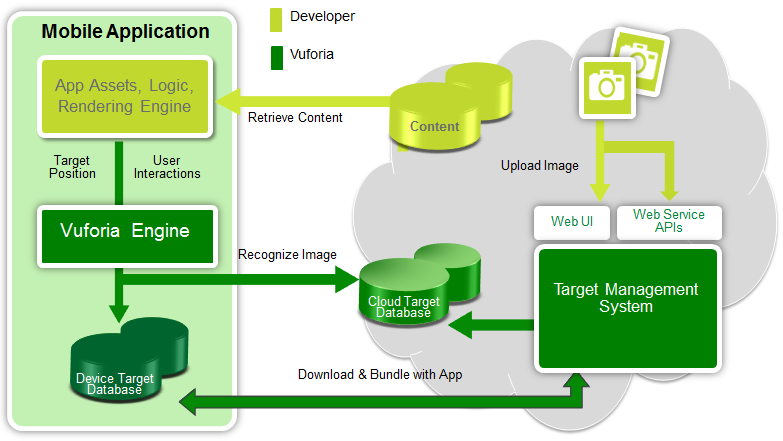
\includegraphics[width=12cm]{imgs/vuforia-components.png}
}

\frame
{
\frametitle{Vuforia: ventajas e inconvenientes}
\begin{itemize}
\item \textbf{Ventajas:}
  \begin{itemize}
   \item Licencia QTL: gratuito y puede usarse en apps comerciales
   \item Gran rendimiento
   \item Posibilidad de reconocimiento en la nube
   \item Clases más sencillas que en OpenCV
  \end{itemize}

\item \textbf{Inconvenientes:}
  \begin{itemize}
   \item Dependencia de NDK + JNI. Si se quiere ampliar, se amplían los métodos nativos.
   \item Cloud recognition no es totalmente gratuito y no podemos montar nuestro propio server
   \item Se centra en visión por computador, así que no tenemos la parte GPS
   \item Foro de debate, con menor orientación a comunidad
  \end{itemize}

\end{itemize}
}

\frame
{
\frametitle{Vuforia: recursos}
\begin{itemize}
\item \textbf{Descarga SDK:} \url{https://developer.vuforia.com/resources/sdk/android}
\item \textbf{Instalación SDK:} \\\url{https://developer.vuforia.com/resources/dev-guide/step-2-installing-vuforia-sdk}
\item \textbf{Target Manager:} \url{https://developer.vuforia.com/targetmanager/project/checkDeviceProjectsCreated?dataRequestedForUserId=}
\item \textbf{Sample apps:} \url{https://developer.vuforia.com/resources/sample-apps}
\item \textbf{Plan de precios Cloud:} \url{https://developer.vuforia.com/cloud-recognition-service}
\end{itemize}
}
